\documentclass[11pt]{article}

\usepackage[margin=1in]{geometry}
\usepackage{amsmath,amssymb,amsthm}
\usepackage{booktabs}
\usepackage{enumitem}
\usepackage{hyperref}
\usepackage{graphicx}
\usepackage{placeins}
\usepackage{xcolor}

\hypersetup{
  colorlinks=true,
  linkcolor=blue,
  citecolor=blue,
  urlcolor=blue
}

\newtheorem{theorem}{Theorem}
\newtheorem{definition}{Definition}
\newtheorem{proposition}{Proposition}
\newtheorem{remark}{Remark}

\newcommand{\R}{\mathbb{R}}
\newcommand{\E}{\mathbb{E}}
\newcommand{\Cov}{\operatorname{Cov}}
\newcommand{\rank}{\operatorname{rank}}
\newcommand{\spanop}{\operatorname{span}}
\newcommand{\chol}{\operatorname{chol}}

\title{Technical Note: Task-Visible Operator Mechanisms\\
for In-Context Linear Ridge Regression}
\author{Fernando Ruiz Mazo}
\date{April 30, 2026}

\begin{document}

\maketitle

\section{Introduction}

The goal is to test whether a trained transformer implements the linear-kernel ridge-regression
operator, not just whether it predicts one label vector correctly. This distinction matters because
many different algorithms can agree on one sampled label vector while responding differently to
nearby label perturbations. We therefore turn each episode into an operator test: freeze the inputs
and ask how predictions change as the context labels are varied.

Fix one episode and hold all non-label inputs fixed:
\[
G = (X_{\mathrm{ctx}}, X_{\mathrm{tgt}}).
\]
Let
\[
X_{\mathrm{ctx}} \in \R^{n_{\mathrm{ctx}}\times d_x},
\qquad
X_{\mathrm{tgt}} \in \R^{n_{\mathrm{tgt}}\times d_x}.
\]
The transformer receives the fixed sequence
\[
(x_1,y_1,0),\ldots,(x_{n_{\mathrm{ctx}}},y_{n_{\mathrm{ctx}}},0),
(x^\star_1,0,1),\ldots,(x^\star_{n_{\mathrm{tgt}}},0,1),
\]
where the first block contains context tokens and the second block contains target tokens. In the
operator tests, only the context-label entries \(y_1,\ldots,y_{n_{\mathrm{ctx}}}\) are perturbed. Rows of
\(X_{\mathrm{ctx}}\) and \(X_{\mathrm{tgt}}\) are sampled from a Gaussian input law. Conditional on an
episode covariance \(\Sigma\),
\[
x_i \sim \mathcal{N}(0,\Sigma), \qquad \Sigma = U\Lambda U^\top,
\]
where \(U\) is a random orthogonal matrix obtained by QR-orthogonalizing a Gaussian matrix. During
training, \(\Lambda\) is sampled from the spectral curriculum described in the experimental setup. The
operator experiments reported below instead use the flat-spectrum evaluation geometry
\[
\Sigma = cI,\qquad c\sim \mathrm{Unif}[1,10],
\]
implemented by the shared flat eigenvalues sampler. Set
\[
K := X_{\mathrm{ctx}}X_{\mathrm{ctx}}^\top,\qquad
K_t := X_{\mathrm{tgt}}X_{\mathrm{ctx}}^\top,\qquad
A := K+\sigma^2 I_{n_{\mathrm{ctx}}},\qquad \sigma^2>0.
\]
These matrices are introduced because, once the inputs are fixed, all of ridge regression is encoded
by the context Gram matrix \(K\), the target-context Gram matrix \(K_t\), and the regularized system
matrix \(A\). Labels are generated by a sampled teacher,
\[
\beta\sim \mathcal{N}(0,I_{d_x}),\qquad
y=X_{\mathrm{ctx}}\beta+\eta,\qquad
\eta\sim \mathcal{N}(0,\sigma^2 I_{n_{\mathrm{ctx}}}).
\]
The target values used for evaluation are the noiseless teacher values \(X_{\mathrm{tgt}}\beta\). This is
the same sampling convention used by the experiment scripts: context labels are noisy, target labels
are not given to the transformer, and KRR is evaluated as the conditional predictor from context
labels to target values. Ridge regression does not observe \(\beta\). It forms its estimate from the
sampled inputs and context labels. For context labels \(y\in\R^{n_{\mathrm{ctx}}}\), exact linear-kernel
ridge regression gives
\[
\alpha^\star=A^{-1}y,\qquad y^\star=K_t\alpha^\star.
\]
Equivalently, after the geometry is fixed, ridge regression is the conditional operator
\[
T_G:=K_tA^{-1},\qquad y^\star=T_Gy.
\]
Equivalently, in primal form,
\[
\widehat{\beta} =
\left(X_{\mathrm{ctx}}^\top X_{\mathrm{ctx}}+\sigma^2 I_{d_x}\right)^{-1}
X_{\mathrm{ctx}}^\top y,
\qquad
y^\star=X_{\mathrm{tgt}}\widehat{\beta}.
\]
Every behavioral, representational, and causal test below is ultimately scored against this operator,
not only against the realized prediction \(T_Gy\).

Let the trained transformer define the fixed-geometry label map
\[
F_\theta^G:\R^{n_{\mathrm{ctx}}}\to \R^{n_{\mathrm{tgt}}},\qquad
F_\theta^G(y)=\widehat{y}_\theta.
\]
When the geometry is clear, we write \(F\) and \(T\) for \(F_\theta^G\) and \(T_G\). The central
comparison is therefore between two maps with the same input and output spaces: the transformer's
local label-response map \(F\) and the exact KRR operator \(T\).

A context-label direction is a vector \(u\in \R^{n_{\mathrm{ctx}}}\) added to the context labels while
the input geometry \(G\) is held fixed. Testing a direction means comparing the transformer's
response to \(y+\varepsilon u\) and \(y-\varepsilon u\). Thus the word ``direction'' always refers to a
direction in label space over the context positions, not to a direction in input-feature space or
target space.

The transformer's activations are the hidden states produced by the trained transformer on the
same fixed episode. When we speak about an activation subspace, we mean a subspace over context
positions extracted from context-token hidden states. Later sections define how these subspaces
are tested against the ridge operator.

This note separates the mechanism claim into three tests.
\begin{enumerate}[label=\arabic*.]
\item \textbf{Behavior.} Does the transformer's local response to label changes match \(T\) on held-out perturbations?
\item \textbf{Representation.} Do the transformer's activations contain a compact context-side subspace from which the same operator can be recovered?
\item \textbf{Causal use.} Once the relevant activation directions have been identified, does removing them damage the transformer's response?
\end{enumerate}

The next section defines the rank requirement before inspecting the transformer. It is a rank
result, not a learning guarantee. The experiments then check whether the trained transformer
exposes a subspace meeting that requirement, whether the transformer response agrees with the
operator built from that subspace, and whether the transformer causally relies on the extracted
directions. The claim is local to task-distribution label directions; isotropic probes show that the
transformer's learned response drifts off distribution.

All theoretical claims are for the linear kernel. The studied transformer is bidirectional, so the
explanation is for the conditional prediction operator \(K_tA^{-1}\), not for a target-independent
stored dual solution.

\paragraph{High-level construction.}
The construction has one organizing idea. After the input geometry is fixed, ridge regression is a
linear map from context labels to target predictions. We want to know whether the transformer
realizes this map through a small context-side activation subspace. The plan is:
\begin{enumerate}[label=\arabic*.]
\item First define the ideal subspace problem without using the transformer: what is the smallest
context-label subspace that can reproduce the ridge operator on task-distributed label directions?
\item Then extract candidate subspaces from the trained transformer's activations and test whether
they are sufficient for the same ridge operator.
\item Finally test three things separately: whether the transformer response matches ridge regression,
whether the extracted subspace is sufficient for ridge regression, and whether the transformer
causally depends on the extracted directions.
\end{enumerate}
Thus the main claim is: the transformer contains a low-dimensional activation subspace whose
dimension matches the rank requirement defined below for the ridge operator; the operator built from
that subspace is accurate; and removing the relevant extracted directions damages the transformer's
task-local response.

\paragraph{Norms.}
The \(A\)-norm is the geometry induced by the ridge linear system. For \(v\in\R^{n_{\mathrm{ctx}}}\)
and \(M\in\R^{n_{\mathrm{ctx}}\times d}\), define
\[
\|v\|_A:=\sqrt{v^\top Av},\qquad
\|M\|_{A,F}:=\|A^{1/2}M\|_F.
\]
All prediction-space norms are Euclidean or Frobenius norms. A fixed numerical floor
\(\eta_{\mathrm{num}}>0\) appears only in denominators; in experiments \(\eta_{\mathrm{num}}=10^{-12}\).

\paragraph{What is not claimed.}
The pre-transformer theory supplies a rank requirement. It does not say that raw depth, head
count, or width imply ridge behavior. It also does not give an SGD or training guarantee. The
layerwise activation-span diagnostic is a post-training diagnostic of where the relevant directions
appear, not a pre-training architecture budget.

\section{Task-Visible Rank}

This section gives the only pre-transformer theorem used in the paper. It depends only on the
input distribution, the label law, and the desired accuracy. Its purpose is to define the target
that any activation explanation must meet. Before looking inside the transformer, we ask: how
many context-label directions are needed, in principle, to reproduce ridge predictions on the label
directions the task actually produces? This number is the benchmark for the later activation
construction. If the transformer exposes fewer useful directions than this, the proposed subspace
cannot approximate the ridge operator on the task distribution; if it exposes enough, the remaining
question is whether the transformer's local response is close to the corresponding subspace-based
approximation and whether the transformer causally depends on that subspace.

Assume the matched random linear regression task
\[
y=X_{\mathrm{ctx}}\beta+\eta,\qquad
\beta\sim \mathcal{N}(0,\tau^2 I_{d_x}),\qquad
\eta\sim \mathcal{N}(0,\tau^2\sigma^2 I_{n_{\mathrm{ctx}}}).
\]
The experiments use \(\tau=1\); the scale \(\tau\) is included here only to make clear that an overall
label scale does not affect the normalized operator errors below. Here the randomness in
\(X_{\mathrm{ctx}}\) and \(X_{\mathrm{tgt}}\) first samples the geometry \(G\); the randomness in
\(\beta\) and \(\eta\) then samples labels conditional on that geometry. Conditional on the geometry \(G\),
\[
\Cov(y\mid G)=\tau^2 A.
\]
Thus task-label directions are isotropic in the whitened coordinates \(A^{-1/2}y\). Define the
task-visible operator
\[
C_G := K_tA^{-1/2}.
\]
Let \(s_1(G)\ge s_2(G)\ge\cdots\ge 0\) be its singular values. The whitening is the reason \(C_G\)
is the right object. In coordinates where task labels are standard Gaussian, \(C_G\) is exactly the
ridge map from whitened label directions to target predictions. Its singular spectrum therefore
says which task-label directions matter most for prediction.

\begin{definition}[Task-visible rank]
For fixed \(G\) and tolerance \(\epsilon>0\), define
\[
r_{\mathrm{task}}(G;\epsilon)
:=
\min\left\{
r:
\frac{\sum_{i>r}s_i(G)^2}{\sum_i s_i(G)^2+\eta_{\mathrm{num}}}
\le \epsilon^2
\right\}.
\]
For random geometries \(G\sim\mathcal{D}_G\), define
\[
r_{\mathrm{task}}^{\mathrm{hp}}(\epsilon,\delta)
:=
\min\left\{
r:
\mathbb{P}_G\!\left(r_{\mathrm{task}}(G;\epsilon)\le r\right)\ge 1-\delta
\right\}.
\]
\end{definition}

This rank is the number of target-visible ridge directions needed on the task label distribution.
It is a requirement that an activation subspace may or may not meet after training; it is not a raw
architectural budget. For the linear kernel, \(\rank(C_G)\le \rank(X_{\mathrm{ctx}})\le d_x\), so the
theorem below gives a concrete finite-dimensional requirement. On the flat-spectrum full-rank
geometries used in the target-rank sweep, the a priori rank calculation in the experiments verifies
that this requirement is essentially \(d_x\) at the reported tolerance.

The next quantity turns the rank question into an operator approximation question. Suppose
two candidate label-to-prediction maps, \(S_1\) and \(S_2\), are equal on one realized label vector but
differ on other possible label directions. We need a way to say how different they are on the
directions we care about. A probe law \(P\) specifies those directions. For example, the task probe
law samples directions with the same covariance as task labels, while the isotropic law samples all
context-label directions equally.

For a fixed geometry and a probe law \(P\), define the population operator error
\[
E_P(S_1,S_2)
:=
\left(
\frac{
\E_{u\sim P}\|(S_1-S_2)u\|_2^2
}{
\E_{u\sim P}\|Tu\|_2^2+\eta_{\mathrm{num}}
}
\right)^{1/2}.
\]
The expectation is only over the probe direction \(u\); the geometry is already fixed. The numerator
is the mean squared prediction-response discrepancy between \(S_1\) and \(S_2\) on the chosen
directions. The denominator is the mean squared response of the exact ridge operator on the same
directions. Thus \(E_P(S_1,S_2)=0.01\) means that the root-mean-square operator discrepancy is
about one percent of the root-mean-square ridge response under \(P\). This normalization lets the
theorem and the experiments use the same scale, and it prevents directions where ridge has almost
no response from dominating the interpretation.

\begin{theorem}[Task-visible rank theorem]
Fix a geometry \(G\) in the matched linear task. Let \(T=K_tA^{-1}\) and let
\(Q\in\R^{n_{\mathrm{ctx}}\times r}\) be \(A\)-orthonormal, \(Q^\top A Q=I_r\). Define the reduced operator
\[
T_Q:=K_tQQ^\top.
\]
Let \(P_{\mathrm{task}}\) be the task-label probe law \(u\mid G\sim\mathcal{N}(0,A)\); the scalar factor
\(\tau^2\) in the matched label covariance cancels in the normalized error. Then
\[
\min_{Q^\top A Q=I_r} E_{P_{\mathrm{task}}}(T_Q,T)^2
=
\frac{\sum_{i>r}s_i(G)^2}{\sum_i s_i(G)^2+\eta_{\mathrm{num}}},
\]
where \(s_i(G)\) are the singular values of \(C_G=K_tA^{-1/2}\). A minimizer is
\[
Q_r^\star=A^{-1/2}V_{1:r},
\]
where \(V_{1:r}\) are the top right singular vectors of \(C_G\). Consequently, if
\(r\ge r_{\mathrm{task}}(G;\epsilon)\), then there exists an \(r\)-dimensional reduced operator with
\[
E_{P_{\mathrm{task}}}(T_Q,T)\le \epsilon.
\]
If \(r\ge r_{\mathrm{task}}^{\mathrm{hp}}(\epsilon,\delta)\), the same statement holds with probability
at least \(1-\delta\) over sampled geometries.
\end{theorem}

\begin{proof}
Let \(W=A^{1/2}Q\). Then \(W^\top W=I_r\) and
\[
T_Q = K_tA^{-1/2}WW^\top A^{-1/2}.
\]
Write \(u=A^{1/2}z\). Under the task-label probe law, \(z\sim\mathcal{N}(0,I)\). Therefore
\[
Tu=C_Gz,\qquad T_Qu=C_GWW^\top z,
\]
so
\[
(T-T_Q)u=C_G(I-WW^\top)z.
\]
Taking expectation over \(z\) gives
\[
\E\|(T-T_Q)u\|_2^2=\|C_G(I-WW^\top)\|_F^2,
\qquad
\E\|Tu\|_2^2=\|C_G\|_F^2.
\]
The optimization is therefore
\[
\min_{W^\top W=I_r}\|C_G(I-WW^\top)\|_F^2.
\]
By Ky Fan's maximum principle, this residual is minimized by the top right singular vectors of
\(C_G\), and the minimum residual is \(\sum_{i>r}s_i^2\). The high-probability statement follows
from the definition of \(r_{\mathrm{task}}^{\mathrm{hp}}\).
\end{proof}

\begin{remark}[Meaning of the sufficient condition]
The theorem above is a rank theorem for context-side subspaces. It says that an \(A\)-orthonormal trial
space of sufficient task-visible dimension can represent the ridge operator on task-label probes. It
does not say that a transformer learns, exposes, or uses such a space. Those are post-training
questions.
\end{remark}

This leaves the central empirical problem. The theorem tells us what a sufficient context-side
subspace would have to accomplish, but it does not tell us whether the trained transformer has
such a subspace or whether the transformer's predictions depend on it. The next section therefore
converts the rank condition into measurable diagnostics: first compare the transformer's local
label-response map to ridge regression, then compare activation-derived reduced operators to both
the transformer and the exact ridge operator.

\section{Operator Diagnostics and Activation Certificates}

Section 2 defined the ideal trial-space target. This section explains how to test that target in
a trained transformer. The central principle is to freeze the geometry, perturb only labels, and
compare the resulting local response to the operator \(T\). We use local perturbations because the
transformer is nonlinear as a function of the whole token sequence, even if the target algorithm is
linear in the labels after the geometry is fixed.

\begin{definition}[Central finite-difference response]
For step size \(\varepsilon>0\) and direction \(u\in\R^{n_{\mathrm{ctx}}}\), define
\[
D_\varepsilon F(y)[u]
:=
\frac{F(y+\varepsilon u)-F(y-\varepsilon u)}{2\varepsilon}.
\]
\end{definition}
This is the measured label-to-prediction response of the transformer in direction \(u\). If the
transformer locally implements ridge regression, this quantity should be close to \(Tu\) on held-out
label directions.

The population error from Section 2 is the ideal quantity, but experiments only use finitely many
label directions. The next definition is its empirical version. The first error compares a nonlinear
transformer to a fixed linear operator by asking: when the labels are nudged in direction \(u_j\),
does the transformer's measured response agree with what operator \(S\) would have produced on
the same direction? Taking several held-out directions makes this an operator test rather than a
test on the original label vector alone.

\begin{definition}[Operator errors]
Let \(U=\{u_1,\ldots,u_m\}\) be a predeclared set of probe directions. For a fixed linear operator
\(S:\R^{n_{\mathrm{ctx}}}\to\R^{n_{\mathrm{tgt}}}\), define
\[
E_\varepsilon(F,S;U)
:=
\left(
\frac{
\sum_{j=1}^m \|D_\varepsilon F(y)[u_j]-Su_j\|_2^2
}{
\sum_{j=1}^m \|Tu_j\|_2^2+\eta_{\mathrm{num}}
}
\right)^{1/2}.
\]
For two linear operators \(S_1,S_2\), define
\[
E(S_1,S_2;U)
:=
\left(
\frac{
\sum_{j=1}^m \|(S_1-S_2)u_j\|_2^2
}{
\sum_{j=1}^m \|Tu_j\|_2^2+\eta_{\mathrm{num}}
}
\right)^{1/2}.
\]
The corresponding population quantity \(E_P(S_1,S_2)\) was defined in Section 2.
\end{definition}

The first quantity, \(E_\varepsilon(F,S;U)\), is used whenever one side of the comparison is the
trained transformer. If \(S=T\), it measures whether the transformer behaves like exact ridge
regression on the probes. If \(S=T_Q\), it measures whether the transformer's local response is close
to the reduced operator induced by an activation subspace. The denominator is the total
ridge-response energy on the same probe set, so the score is read as a relative root-mean-square
response error. A small value means the discrepancy is small compared with the prediction changes
that ridge regression itself would make on those directions.

The second quantity, \(E(S_1,S_2;U)\), removes the transformer from the comparison and only asks
whether two linear operators act similarly on the same probes. This is why later sections can
separate transformer-to-reduced-operator error, \(E_\varepsilon(F,T_Q)\), from subspace error,
\(E(T_Q,T)\).

Task-distribution probes test the directions emphasized by training; isotropic probes test a
stronger global response. If \(u\sim\mathcal{N}(0,I)\), then \(\E\|Mu\|_2^2=\|M\|_F^2\), so isotropic
Gaussian probes estimate Frobenius operator error.

The operator errors above assume that the transformer has a stable local linear response around
the observed label vector. A small transformer-to-ridge error is hard to interpret if the
finite-difference response changes strongly when two probe directions are combined. The additivity
defect is a guardrail for this issue: it checks whether the local response to \(u+v\) is approximately
the sum of the local responses to \(u\) and \(v\).

\begin{definition}[Additivity defect]
For paired probe directions \(V=\{(u_j,v_j)\}_{j=1}^m\), define
\[
C_j :=
F(y+\varepsilon u_j+\varepsilon v_j)
-F(y+\varepsilon u_j-\varepsilon v_j)
-F(y-\varepsilon u_j+\varepsilon v_j)
+F(y-\varepsilon u_j-\varepsilon v_j),
\]
\[
A_\varepsilon(F;V)
:=
\left(
\frac{
\sum_{j=1}^m\|C_j\|_2^2
}{
\sum_{j=1}^m\|T(\varepsilon u_j+\varepsilon v_j)\|_2^2+\eta_{\mathrm{num}}
}
\right)^{1/2}.
\]
\end{definition}

The four evaluations in \(C_j\) cancel exactly for an affine function of the labels. Thus a small
\(A_\varepsilon(F;V)\) says that, at the chosen scale and probe law, the transformer's local response
is close enough to linear that comparing it to a linear operator is meaningful. A large value would
mean that the transformer may be nonlinear in the neighborhood being probed, so errors such as
\(E_\varepsilon(F,T)\) would mix two effects: failure to be ridge and failure to be locally linear. The
additivity defect is only a validity check for the operator diagnostic; by itself it is not evidence
that the linear operator is the ridge operator.

\subsection{Reduced Operators from Activations}

The behavioral test says whether the transformer response matches ridge regression, but not where
the computation is represented. The next step is to ask whether the context-token activations
define a small trial space from which ridge regression can be reconstructed. This is why the basis
\(Q\) lives on the context-label side rather than in target space.

\begin{definition}[\(A\)-orthonormal trial basis and reduced operator]
A matrix \(Q\in\R^{n_{\mathrm{ctx}}\times r}\) is \(A\)-orthonormal if \(Q^\top AQ=I_r\). The reduced
operator induced by \(Q\) is the linear operator
\[
T_Q:=K_tQQ^\top.
\]
For a general full-rank basis \(Z\in\R^{n_{\mathrm{ctx}}\times r}\), the same operator is
\[
T_Z:=K_tZ(Z^\top AZ)^{-1}Z^\top.
\]
\end{definition}

The reduced operator is the restriction of ridge regression to the trial space. If \(Q^\top AQ=I\),
then the reduced dual vector
\[
\alpha_Q=QQ^\top y
\]
is the \(A\)-orthogonal projection of \(\alpha^\star=A^{-1}y\) onto \(\operatorname{col}(Q)\), and
\[
T-T_Q=K_t(I-QQ^\top A)A^{-1}.
\]
Thus \(T_Q\) is not an arbitrary readout from activations. It is the ridge operator one obtains when
the dual solution is forced to lie in the activation-derived context subspace.

\begin{proposition}[Linear feature trial space]
For the linear kernel, let \(Z\) be any full-rank basis for \(\operatorname{col}(X_{\mathrm{ctx}})\). Then
the reduced operator
\[
T_Z=K_tZ(Z^\top AZ)^{-1}Z^\top
\]
equals the exact operator \(T=K_tA^{-1}\).
\end{proposition}

\begin{proof}
Fix \(y\) and write \(\alpha^\star=A^{-1}y\) and
\[
\alpha_Z=Z(Z^\top AZ)^{-1}Z^\top y.
\]
The restricted normal equations give
\[
Z^\top A(\alpha^\star-\alpha_Z)=0.
\]
Since \(\operatorname{col}(Z)=\operatorname{col}(X_{\mathrm{ctx}})\), this implies
\[
X_{\mathrm{ctx}}^\top A(\alpha^\star-\alpha_Z)=0.
\]
Let \(r=\alpha^\star-\alpha_Z\). Using \(A=X_{\mathrm{ctx}}X_{\mathrm{ctx}}^\top+\sigma^2 I\),
\[
X_{\mathrm{ctx}}^\top Ar
=
(X_{\mathrm{ctx}}^\top X_{\mathrm{ctx}}+\sigma^2 I_{d_x})X_{\mathrm{ctx}}^\top r.
\]
The matrix in parentheses is positive definite, so \(X_{\mathrm{ctx}}^\top r=0\). Therefore
\(K_tr=X_{\mathrm{tgt}}X_{\mathrm{ctx}}^\top r=0\), and \(T_Zy=K_t\alpha_Z=K_t\alpha^\star=Ty\) for
every \(y\).
\end{proof}

\begin{definition}[Frozen extraction map]
A frozen extraction map \(\mathcal{E}\) maps the unperturbed episode and activations to an
\(A\)-orthonormal basis
\[
Q=\mathcal{E}(G,y,\mathrm{activations}).
\]
After \(Q\) is extracted, the reduced operator \(T_Q\) is held fixed when label perturbations are
tested.
\end{definition}

Freezing \(Q\) is essential. Otherwise the basis could change with every probe direction, and the
test would no longer certify one stable reduced operator carried by the unperturbed activations.
In the experiments, this abstract map is instantiated in three concrete ways. Experiment 1 uses
final-state weighted-SVD extractors: a raw extractor from the unperturbed final context hidden
state, and a response-only extractor from final-state finite differences on build probes. Experiment
2 uses the layerwise activation-span extractor, which builds a basis from hidden-state
finite-difference responses after removing directions already explained by earlier layers. Experiment
3 uses the raw final-state extractor from Experiment 1, because the causal intervention removes
directions from the actual residual stream. In all cases the extraction uses only the unperturbed
episode and build probes; evaluation is performed afterward on held-out probes with \(Q\) fixed.

\begin{definition}[Pointwise errors]
For a frozen basis \(Q\), define
\[
e_{\mathrm{sub}}(Q;G,y)
=
\frac{\|T_Qy-Ty\|_2}{\|Ty\|_2+\eta_{\mathrm{num}}},
\qquad
\tau_{\mathrm{read}}(Q;G,y)
=
\frac{\|F(y)-T_Qy\|_2}{\|Ty\|_2+\eta_{\mathrm{num}}}.
\]
Then
\[
\frac{\|F(y)-Ty\|_2}{\|Ty\|_2+\eta_{\mathrm{num}}}
\le
e_{\mathrm{sub}}(Q;G,y)+\tau_{\mathrm{read}}(Q;G,y).
\]
\end{definition}

This pointwise statement is only a sanity check. The operator statement is stronger.

\begin{theorem}[Operator residual decomposition]
For every frozen \(A\)-orthonormal basis \(Q\) and probe set \(U\),
\[
D_\varepsilon F(y)[u]-Tu
=
\underbrace{D_\varepsilon F(y)[u]-T_Qu}_{\text{transformer--reduced-operator residual}}
+
\underbrace{(T_Q-T)u}_{\text{subspace residual}}.
\]
Consequently,
\[
E_\varepsilon(F,T;U)
\le
E_\varepsilon(F,T_Q;U)+E(T_Q,T;U).
\]
\end{theorem}

The two terms answer different questions. The subspace residual \(E(T_Q,T)\) asks whether the
activation subspace is sufficient for the ridge operator. The transformer--reduced-operator residual
\(E_\varepsilon(F,T_Q)\) asks whether the trained transformer's local response is close to the reduced
operator induced by that subspace. These two residuals are the quantities used for the mechanism
claim; auxiliary explained-fraction summaries are computed in the experiment logs but are not
needed for the note's argument.

\subsection{Final-State Extractors}

The final-state extractor is the simplest way to ask whether the computation has left a usable
context-side subspace in the residual stream. The object we need for the reduced operator is a
basis \(Q\in\R^{n_{\mathrm{ctx}}\times r}\): its columns are directions over context positions. The final
context hidden state has exactly this context axis. If \(H_L^{\mathrm{ctx}}\in\R^{n_{\mathrm{ctx}}\times D}\)
is the final context-token hidden-state matrix, then each hidden coordinate gives one
length-\(n_{\mathrm{ctx}}\) pattern across the context tokens. The span of these patterns is the part of
context-label space that is linearly visible in the final context representation.

The extractor measures this visible span and converts it into the kind of basis used by the
reduced operator. For any matrix \(M\in\R^{n_{\mathrm{ctx}}\times p}\) whose columns are context-token
patterns, compute
\[
A^{1/2}M=U\Sigma V^\top.
\]
We keep the left singular directions whose singular values are at least \(\tau_{\mathrm{sv}}\sigma_1\),
up to the cap \(r_{\max}\), and set
\[
Q(M):=A^{-1/2}U_{\mathrm{kept}}.
\]
This guarantees \(Q(M)^\top A Q(M)=I\). The \(A^{1/2}\) weighting is not a cosmetic choice: the
ridge system measures dual directions using \(A\), so the extractor ranks activation patterns by
size in the same geometry in which \(T_Q=K_tQQ^\top\) is defined.

Experiment 1 uses two choices of \(M\). The response-only choice is built from task-label build
directions and then held fixed when we test both task-label and isotropic evaluation probes.

The raw extractor uses
\[
M_{\mathrm{raw}}=H_L^{\mathrm{ctx}},
\qquad
Q_L^{\mathrm{raw}}:=Q(M_{\mathrm{raw}}).
\]
This asks a broad availability question: does the final context state contain some subspace from
which the ridge operator can be reconstructed?

The response-only extractor uses hidden-state changes caused by label perturbations. For build
probes \(u\in U_{\mathrm{build}}\), define
\[
Z_L(u)=
\frac{
H_L^{\mathrm{ctx}}(y+\varepsilon u)-H_L^{\mathrm{ctx}}(y-\varepsilon u)
}{2\varepsilon},
\]
and stack these matrices as
\[
M_{\mathrm{resp}}=[Z_L(u_1),\ldots,Z_L(u_m)],
\qquad
Q_L^{\mathrm{resp}}:=Q(M_{\mathrm{resp}}).
\]
This asks a stricter question: do the label-sensitive final-state directions contain a subspace whose
reduced operator is close to ridge regression?

After either basis is extracted, it is frozen. The experiment then computes the reduced operator
\(T_Q=K_tQQ^\top\) and measures two held-out quantities: \(E(T_Q,T)\), which tests whether the
extracted subspace is sufficient for ridge, and \(E_\varepsilon(F,T_Q)\), which tests whether the
transformer's local response is close to the reduced operator induced by that subspace.

For a bidirectional transformer, these bases may be target-conditioned. The claim is therefore
about the conditional prediction operator \(K_tA^{-1}\).

The final-state certificate is enough to test whether a suitable subspace is present at the end of
the computation. It is not enough to say how that subspace arises across layers. The next section
introduces a stricter diagnostic for that question.

\section{Layerwise Activation Span}

The final-state certificate says whether a useful subspace is present at the end of the computation.
It does not say whether that subspace can be traced to label-sensitive changes that appear during
the layers. This section builds a layerwise activation span for that purpose. The diagnostic is
deliberately post-training: it measures what the trained transformer exposes, not what depth,
width, or head count should guarantee.

The construction keeps only directions that move when the context labels are perturbed. Fix
build probes \(U_{\mathrm{build}}=\{u_1,\ldots,u_m\}\). Let \(H_\ell^{\mathrm{ctx}}(y)\) be the context-token
hidden-state matrix after layer \(\ell\), and define the finite-difference hidden response
\[
Z_\ell(u):=
\frac{
H_\ell^{\mathrm{ctx}}(y+\varepsilon u)-H_\ell^{\mathrm{ctx}}(y-\varepsilon u)
}{2\varepsilon}.
\]
Stack the build-probe responses as
\[
M_\ell=[Z_\ell(u_1),\ldots,Z_\ell(u_m)].
\]
The columns of \(M_\ell\) are context-position patterns that are visible in layer \(\ell\) when labels
move. A direction that does not appear in these finite differences is not counted as evidence for a
label-computation mechanism.

We now accept new directions one layer at a time. If \(Q\) is an \(A\)-orthonormal basis of a
subspace, the \(A\)-orthogonal projection of a matrix \(M\) onto that subspace is
\[
P_Q^A M := QQ^\top AM.
\]
Before processing layer \(\ell\), suppose that the accepted direction matrices \(S_0,\ldots,S_{\ell-1}\)
have already been constructed. Each \(S_j\) has \(A\)-orthonormal columns and represents directions
first accepted at layer \(j\). The directions already available before layer \(\ell\) are
\[
R_\ell^{\mathrm{pre}}
:=
\spanop\{A^tS_j:0\le j<\ell,\ 0\le t\le \ell-j\}.
\]
For \(\ell=0\) this space is empty. The powers of \(A\) are an accounting device: a direction accepted
earlier has more remaining layers in which it could be refined in the ridge-system geometry. We
do not need to claim that the network literally multiplies by \(A\) at each layer; the point is to
avoid counting as new a direction that is already obtainable from earlier accepted directions under
the same geometry used by the reduced operator.

Let \(Q_\ell^{\mathrm{pre}}\) be an \(A\)-orthonormal basis of \(R_\ell^{\mathrm{pre}}\). Remove the part of the
layer response that is already explained by this earlier space:
\[
N_\ell
:=
M_\ell-P_{Q_\ell^{\mathrm{pre}}}^AM_\ell
=
\left(I-Q_\ell^{\mathrm{pre}}(Q_\ell^{\mathrm{pre}})^\top A\right)M_\ell.
\]
Thus \(N_\ell\) is the novel label-sensitive part of layer \(\ell\).

Candidate directions for layer \(\ell\) are obtained by an \(A\)-weighted SVD of \(N_\ell\). This means
computing
\[
A^{1/2}N_\ell=U_\ell\Sigma_\ell V_\ell^\top.
\]
The left singular vectors with \(\sigma_i\ge \tau_{\mathrm{sv}}\sigma_1\) are the candidates. A declared
selection rule then chooses an index set \(I_\ell\) of these candidates, with \(s_\ell=|I_\ell|\). The
experiment below uses a causal selection rule: a candidate is accepted only if removing it from the
context residual stream changes the transformer's local response by a predeclared amount. If the
accepted indices are \(I_\ell\), define
\[
S_\ell:=A^{-1/2}U_{\ell,I_\ell}.
\]
Then \(S_\ell^\top AS_\ell=I\). The \(A\)-weighting matters because the reduced operator and the
ridge dual variables are measured in the \(A\)-geometry. This SVD is therefore principal-component
extraction in the geometry relevant to the ridge system, not in the raw Euclidean geometry of
hidden states.

After the last layer \(L\), define the layerwise activation span
\[
R_{\mathrm{lay}}
:=
\spanop\{A^tS_\ell:0\le \ell\le L,\ 0\le t\le L-\ell\},
\qquad
d_{\mathrm{lay}}:=\dim R_{\mathrm{lay}}.
\]
Let \(Q_{\mathrm{lay}}\) be an \(A\)-orthonormal basis of \(R_{\mathrm{lay}}\). The reduced operator induced by
the layerwise span is
\[
T_{Q_{\mathrm{lay}}}=K_tQ_{\mathrm{lay}}Q_{\mathrm{lay}}^\top.
\]
We also report the upper count
\[
B_{\mathrm{lay}}:=\sum_{\ell=0}^Ls_\ell(L-\ell+1),
\qquad
d_{\mathrm{lay}}\le B_{\mathrm{lay}}.
\]
This count is not an architecture budget. It is only the number of candidate directions produced
by the accounting procedure before linear dependencies are removed.

The span is useful only if it actually covers the layer responses it is meant to explain. For each
layer \(k\), define the partial span
\[
R_k:=\spanop\{A^tS_\ell:0\le \ell\le k,\ 0\le t\le k-\ell\},
\]
and let \(Q_k\) be an \(A\)-orthonormal basis of \(R_k\). The closure defect is
\[
\delta_k^{\mathrm{close}}
:=
\frac{
\|(I-Q_kQ_k^\top A)M_k\|_{A,F}
}{
\|M_k\|_{A,F}+\eta_{\mathrm{num}}
}.
\]
A small closure defect means that the accepted directions up to layer \(k\) can reconstruct the
label-sensitive response observed at layer \(k\). A large closure defect means that the final span
may still work as an endpoint certificate, but the proposed layerwise account is missing much of
the hidden response it claims to summarize.

The refinement fraction is an auxiliary diagnostic for how much a layer reuses directions accepted
earlier. For \(k\ge 1\), let
\[
B_k:=\spanop(R_{k-1}\cup AR_{k-1}),
\]
and let \(Q_k^{\mathrm{ref}}\) be an \(A\)-orthonormal basis of \(B_k\). Define
\[
\rho_k^A
:=
\frac{
\|Q_k^{\mathrm{ref}}(Q_k^{\mathrm{ref}})^\top AM_k\|_{A,F}
}{
\|M_k\|_{A,F}+\eta_{\mathrm{num}}
},
\qquad
\rho_0^A:=0.
\]
Large \(\rho_k^A\) means that much of layer \(k\)'s label response is already explained by previous
directions plus one additional \(A\)-refinement. Small \(\rho_k^A\) means that the layer response is
mostly treated as new information. The main operator claim does not rely on this fraction; it is
reported to separate reuse of earlier streams from genuinely new layerwise directions.

Experiment 2 tests the following post-training hypothesis:
\[
d_{\mathrm{lay}}/r_{\mathrm{task}}\approx 1
\quad\Longrightarrow\quad
E_{P_{\mathrm{task}}}(T_{Q_{\mathrm{lay}}},T)\approx 0,
\]
provided the closure defects are small. Agreement between the transformer response and the
layerwise span is tested separately by \(E_\varepsilon(F,T_{Q_{\mathrm{lay}}})\).

The high-level idea is now clear. The task-visible rank theorem says that ridge regression does
not need all possible context-label directions: under task-label probes, it can be represented by a
low-dimensional context-side space. The layerwise diagnostic asks whether the transformer appears
to build such a space in its context-token activations. If it does, then label perturbations should
reveal only a small number of directions, most later responses should be refinements or reuse of
earlier directions, and the final span should induce a reduced operator close to exact ridge
regression. The desired evidence is therefore simultaneous: \(d_{\mathrm{lay}}\) should be close to
\(r_{\mathrm{task}}\), \(T_{Q_{\mathrm{lay}}}\) should have small operator error, and the closure defects should
be small. This combination would mean that the activation span is not merely a post hoc low-rank
fit at the output; it is also consistent with the transformer carrying the task-relevant context-label
degrees of freedom through its layers.

At this point we have a behavioral test, an endpoint subspace certificate, and a layerwise
activation-span diagnostic. The experiments now apply these objects in order. Experiment 1 tests
behavior and the final-state certificate, including its low-rank alternative. Experiment 2 tests the
layerwise span against the task-visible rank. Experiment 3 tests whether the directions that the
reduced operator ranks as important are causally used.

\section{Experiments}

The experiments follow the certificate in order. The common design principle is to separate
construction from evaluation: subspaces and fitted controls are built from one probe set, while
numerical claims are reported on held-out label directions. This is the experimental analogue of
freezing \(Q\) in the theory. The experiments are therefore not three independent demonstrations.
They are a sequence of checks that close the gaps left by the theorem: behavior first,
representation second, and causal use third.

\subsection{Experimental Setup}

\paragraph{Transformer checkpoint.}
Unless otherwise stated, we use checkpoint \texttt{model\_L8.pt}: an 8-layer bidirectional
transformer with \(d_x=5\), width \(D=128\), 4 attention heads, two-layer GELU FFNs, residual
connections, no LayerNorm, no positional encodings, and a linear readout on target tokens.

\paragraph{Training distribution.}
Each training episode samples a fresh linear regression task. The input covariance is
\(\Sigma=U\Lambda U^\top\), with \(U\) drawn by QR-orthogonalizing a Gaussian matrix and
\(\Lambda\) drawn uniformly from three spectral families: polynomial decay, exponential decay, and
step spectra. Labels are \(y=x^\top\beta+\epsilon\) with \(\beta\sim\mathcal{N}(0,I)\) and
\(\epsilon\sim\mathcal{N}(0,\sigma^2)\), using \(\sigma^2=0.1\). Training uses 50 points per episode
with \(n_{\mathrm{tgt}}\sim\mathrm{Unif}\{1,\ldots,10\}\) and
\(n_{\mathrm{ctx}}=50-n_{\mathrm{tgt}}\).

\paragraph{Evaluation geometry.}
The operator experiments use the linear kernel \(K=XX^\top\) and \(A=K+\sigma^2I\).
``Flat-spectrum OOD'' means that the covariance eigenvalues are all equal to one random scale
\(c\sim\mathrm{Unif}[1,10]\); this spectrum is not present in training. Experiments 1--3 use
\(n_{\mathrm{ctx}}=47\) context points. Experiment 1 uses \(n_{\mathrm{tgt}}=3\); Experiments 2--3 use
\(n_{\mathrm{tgt}}=16\).

\paragraph{Probe and extraction settings.}
All finite differences use \(\varepsilon=10^{-3}\) and numerical floor \(10^{-12}\). Weighted-SVD
extraction uses \(\tau_{\mathrm{sv}}=10^{-3}\). For a fixed episode geometry, task-label probes are
sampled as \(u\sim\mathcal{N}(0,A)\), implemented as \(u=z\,\chol(A)^\top\) with
\(z\sim\mathcal{N}(0,I_{n_{\mathrm{ctx}}})\). Isotropic stress probes are sampled as
\(u\sim\mathcal{N}(0,I_{n_{\mathrm{ctx}}})\). The interpolation sweep uses independent draws
\[
u_\lambda=(1-\lambda)^{1/2}u_{\mathrm{task}}+\lambda^{1/2}u_{\mathrm{iso}},
\]
so its covariance is \((1-\lambda)A+\lambda I_{n_{\mathrm{ctx}}}\). Experiment 1 uses 4 episodes,
16 build probes, 32 held-out evaluation probes, 4 additivity probe pairs, and \(r_{\max}=L+1=9\).
Experiment 2 uses 16 episodes per setting, 16 build probes, 16 hidden-validation probes,
8 causal-selection probes, 16 held-out evaluation probes, causal damage threshold 0.05, and at
most 16 SVD candidates per layer. It includes depth checkpoints \(L\in\{2,4,6,8,12\}\), head
checkpoints \(H\in\{1,2,8\}\), and input-dimension checkpoints
\(d_x\in\{3,5,8,10,15\}\). Experiment 3 uses 32 episodes, 32 causal probes, \(r_{\max}=12\), and
removes \(k\in\{1,2,4\}\) directions. Auxiliary rank checks use 1024 sampled geometries per
\(d_x\) at \((\epsilon,\alpha)=(0.01,0.05)\). Reported random seeds are 123 for Experiment 1 and
42 for Experiments 2--3.

The setup deliberately uses flat-spectrum evaluation geometries for the operator experiments.
This makes the rank requirement easy to interpret and keeps the geometry separate from the
spectral curriculum used in training. Task-label probes then test the label directions induced by
the sampled evaluation geometry. Experiment 1 also includes isotropic probes as a stricter stress
test; Experiments 2--3 report task-label probes because their claim is task-local.

\subsection{Experiment 1: Final-State Operator Certificate}

\paragraph{Question.}
Does the transformer locally behave like exact KRR, and if so, can that behavior be explained
through a subspace visible in the final context-token activation state? The first test is behavioral:
on held-out label perturbations, is \(D_\varepsilon F(y)\) close to the exact ridge operator \(T\)?
Only after that test passes does it make sense to ask whether the agreement factors through an
activation-derived reduced operator.

For any frozen basis \(Q\), the operator residual decomposes as
\[
D_\varepsilon F(y)[u]-Tu
=
\bigl(D_\varepsilon F(y)[u]-T_Qu\bigr)+(T_Q-T)u.
\]
Thus Experiment 1 is organized around three checks. First, the transformer should be close to
exact KRR: \(E_\varepsilon(F,T)\) should be small. Second, the reduced operator \(T_Q\) should be
close to exact KRR. Third, the transformer should be close to \(T_Q\). If only the first condition
held, we would have behavior without a representation certificate. If only \(T_Q\approx T\) held,
the subspace would be sufficient for KRR but not tied to the transformer's response. If only
\(F\approx T_Q\) held, the transformer and the subspace could agree on the wrong operator.

\paragraph{Procedure.}
For each episode, fix \(G\) and compute \(A\), \(T=K_tA^{-1}\), and \(Ty\). Draw task-label build
probes and held-out evaluation probes. Extract \(Q_L^{\mathrm{raw}}\) and \(Q_L^{\mathrm{resp}}\). Here
\(Q_L^{\mathrm{raw}}\) is the basis extracted from the unperturbed final context-token hidden-state
matrix \(H_L^{\mathrm{ctx}}\): it uses all context-side directions visible in the final activation state.
\(Q_L^{\mathrm{resp}}\) is extracted instead from finite-difference changes of that final hidden state
under task-label build perturbations: it keeps only directions that move when the context labels
are changed along directions generated by the task. Both bases are then frozen. We evaluate them
on held-out task-label probes and on held-out isotropic probes; the isotropic rows are therefore a
transfer test of the task-extracted bases, not a new isotropic extraction. For each basis, form the
reduced operator \(T_Q=K_tQQ^\top\).

The comparison control is a same-span response-fitted low-rank operator. It uses the same
context-side features \(Q^\top u\) as the reduced operator, but it does not use the KRR coefficients
\(K_tQ\). Instead, it fits a free target-side coefficient matrix to the transformer's finite-difference
responses on build probes:
\[
C_Q \in
\arg\min_{C\in\R^{n_{\mathrm{tgt}}\times r}}
\sum_{u\in U_{\mathrm{build}}}
\|D_\varepsilon F(y)[u]-CQ^\top u\|_2^2,
\qquad
T_{\mathrm{actLR}}:=C_QQ^\top.
\]
Thus, on a new perturbation \(u\), \(T_{\mathrm{actLR}}u\) first computes the same coordinates
\(Q^\top u\) and then maps those coordinates to target responses using the fitted matrix \(C_Q\).
The subscript actLR abbreviates ``activation-span low-rank response fit.'' This control answers a
decodability question: using the same subspace coordinates, how well can a freely fitted target-side
map reproduce the transformer's local responses? It is not the KRR certificate, because its
target-side coefficients are chosen from the transformer rather than from the KRR geometry. Then
evaluate \(T\), \(T_Q\), and \(T_{\mathrm{actLR}}\) on held-out probes. The reported comparison also
includes random \(A\)-orthonormal subspaces of the same rank; these fail by one to two orders of
magnitude on task probes and are used only to exclude the explanation that any subspace of the
same dimension would suffice.

\paragraph{Results.}
The first check passes: the transformer is already close to exact KRR on the task-local perturbations
we care about. On the sampled task labels, the transformer has MSE 0.0161 against the noiseless
teacher targets, while exact KRR has MSE 0.0148; the ratio is 1.188. The pointwise relative
transformer--KRR discrepancy is 0.01045. On held-out task-label perturbations, the finite-difference
transformer--KRR error is \(E_\varepsilon(F,T)=0.0121\). This establishes the behavioral target
that the rest of the experiment tries to explain through final activations. Additivity defects are
much smaller than the operator errors: \(4.4\times10^{-4}\) on task probes and \(3.5\times10^{-3}\)
on isotropic probes at \(\varepsilon=10^{-3}\), with the same scale at \(10\varepsilon\).

\begin{table}[ht]
\centering
\caption{Behavioral KRR check for the trained transformer, mean over 4 episodes. The operator
error is measured on held-out task-label perturbations.}
\begin{tabular}{lccc}
\toprule
Quantity & Transformer & Exact KRR & Transformer--KRR\\
\midrule
Pointwise MSE to teacher targets & 0.0161 & 0.0148 & --\\
Pointwise relative discrepancy & -- & -- & 0.01045\\
Held-out operator error \(E_\varepsilon(F,T)\) & -- & -- & 0.0121\\
\bottomrule
\end{tabular}
\end{table}

We then ask whether this behavioral agreement can be explained through the final activation
subspaces.

\begin{table}[ht]
\centering
\caption{Reduced operator vs. same-span response-fitted low-rank control, mean over 4 episodes.
\(E(F,S)\) denotes transformer-to-\(S\) operator error; \(E(S,T)\) denotes \(S\)-to-ridge operator error.}
\begin{tabular}{llcccc}
\toprule
Probe distribution & Basis & \(E(F,T_Q)\) & \(E(F,T_{\mathrm{actLR}})\) & \(E(T_Q,T)\) & \(E(T_{\mathrm{actLR}},T)\)\\
\midrule
Task probes & raw & 0.01194 & 0.00726 & 0.00148 & 0.01202\\
Task probes & response & 0.01239 & 0.01169 & 0.00367 & 0.01645\\
Isotropic probes & raw & 0.2915 & 0.2007 & 0.05254 & 0.2687\\
Isotropic probes & response & 0.3193 & 0.2418 & 0.1278 & 0.2929\\
\bottomrule
\end{tabular}
\end{table}

The raw final-state basis gives the cleanest certificate. On task probes, \(T_Q\) is very close to
exact KRR \((E(T_Q,T)=0.00148)\), and the transformer is close to \(T_Q\)
\((E(F,T_Q)=0.01194)\). The response-fitted control fits the transformer slightly better
\((0.00726)\), but it is much farther from exact KRR \((0.01202)\). This does not make the
control a failure; it shows that optimizing the readout for transformer fit is a different question
from certifying that the same subspace supports the KRR operator. The response-only basis gives
the same task-probe pattern, with \(T_Q\) still close to KRR \((0.00367)\) and the response-fitted
control farther from KRR \((0.01645)\).

Random subspaces of the same ranks do not explain the result. On task probes, the raw random
control has \(E(T_Q,T)=0.117\) and \(E(F,T_Q)=0.118\), roughly two orders of magnitude worse
than the raw final-state basis. The response random control is similar, with \(E(T_Q,T)=0.0955\)
and \(E(F,T_Q)=0.0955\).

The result is task-local. At the isotropic endpoint, the transformer--KRR operator error rises to
about 0.302. For the raw basis, the reduced operator also degrades but remains closer to KRR than
the transformer response: \(E(T_Q,T)=0.0525\) while \(E(F,T_Q)=0.292\). The task-built
response-only basis also degrades off task: \(E(T_Q,T)=0.128\) and \(E(F,T_Q)=0.319\) on
isotropic probes. Thus the response basis is useful as a task-local certificate, but it is not a global
explanation of arbitrary label directions. The interpolation sweep in Figure~\ref{fig:interpolation}
shows this transition from task-label directions to isotropic directions.

\begin{figure}[!htbp]
\centering
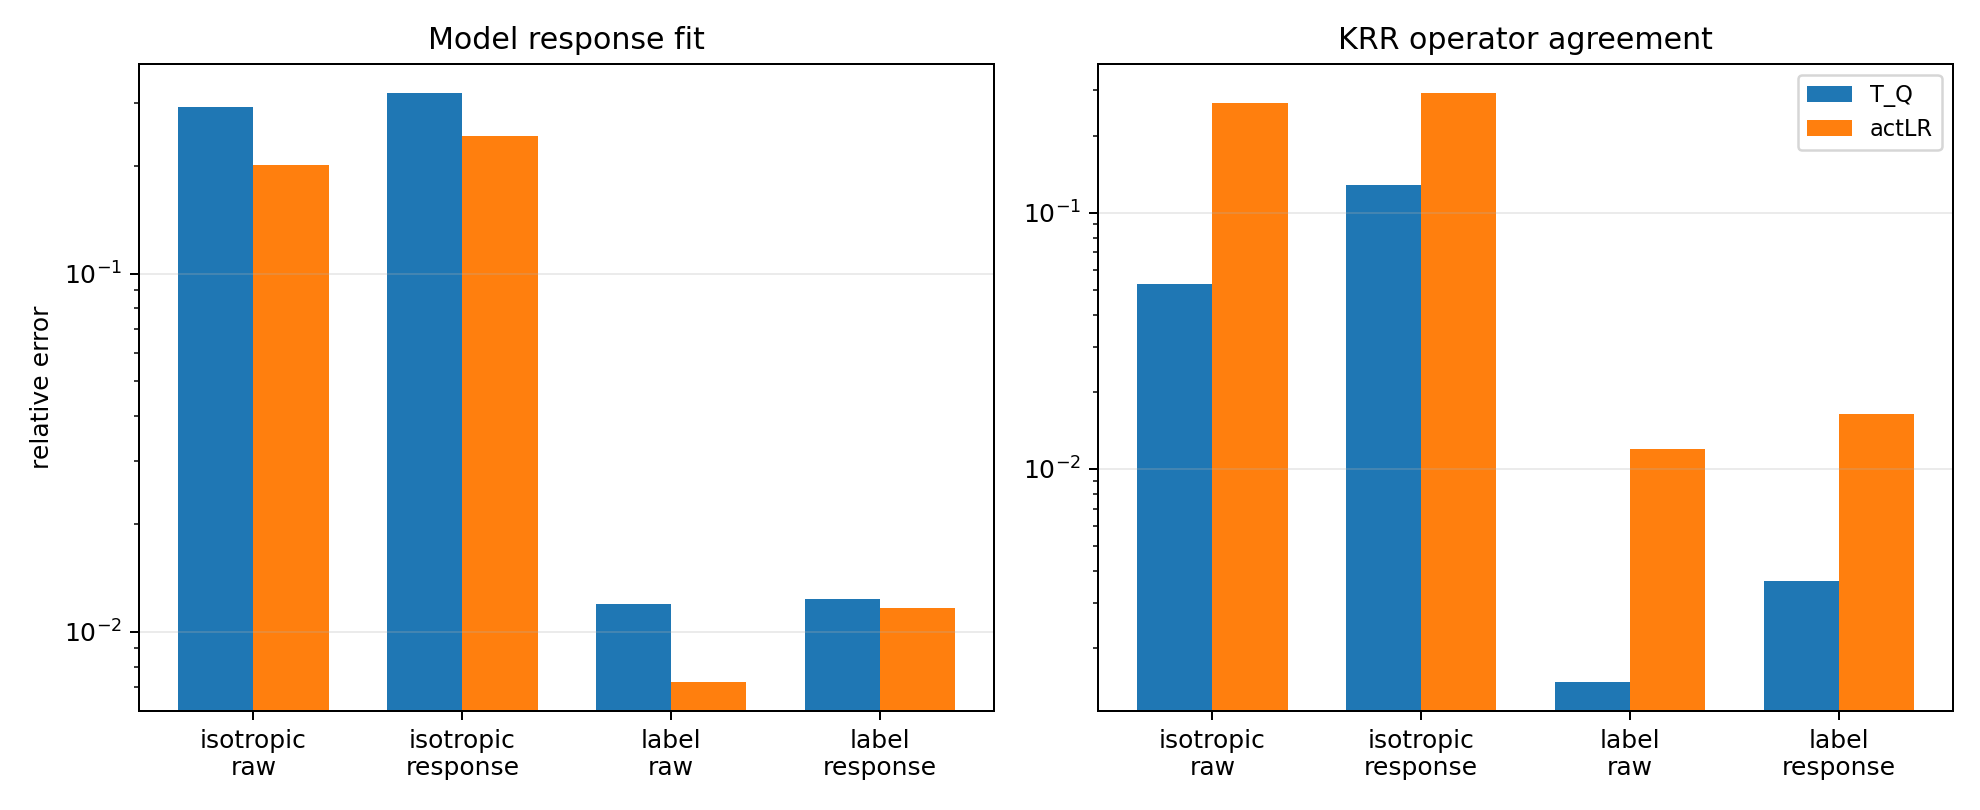
\includegraphics[width=\linewidth]{../experiments/exp1_operator_certificate/results/actlr_comparison.png}
\caption{Reduced operator \(T_Q\) vs. the same-span response-fitted low-rank control
\(T_{\mathrm{actLR}}\). On task probes, the response-fitted control fits the transformer slightly
better but agrees substantially worse with the ridge operator.}
\label{fig:reduced-vs-control}
\end{figure}

\begin{figure}[!htbp]
\centering
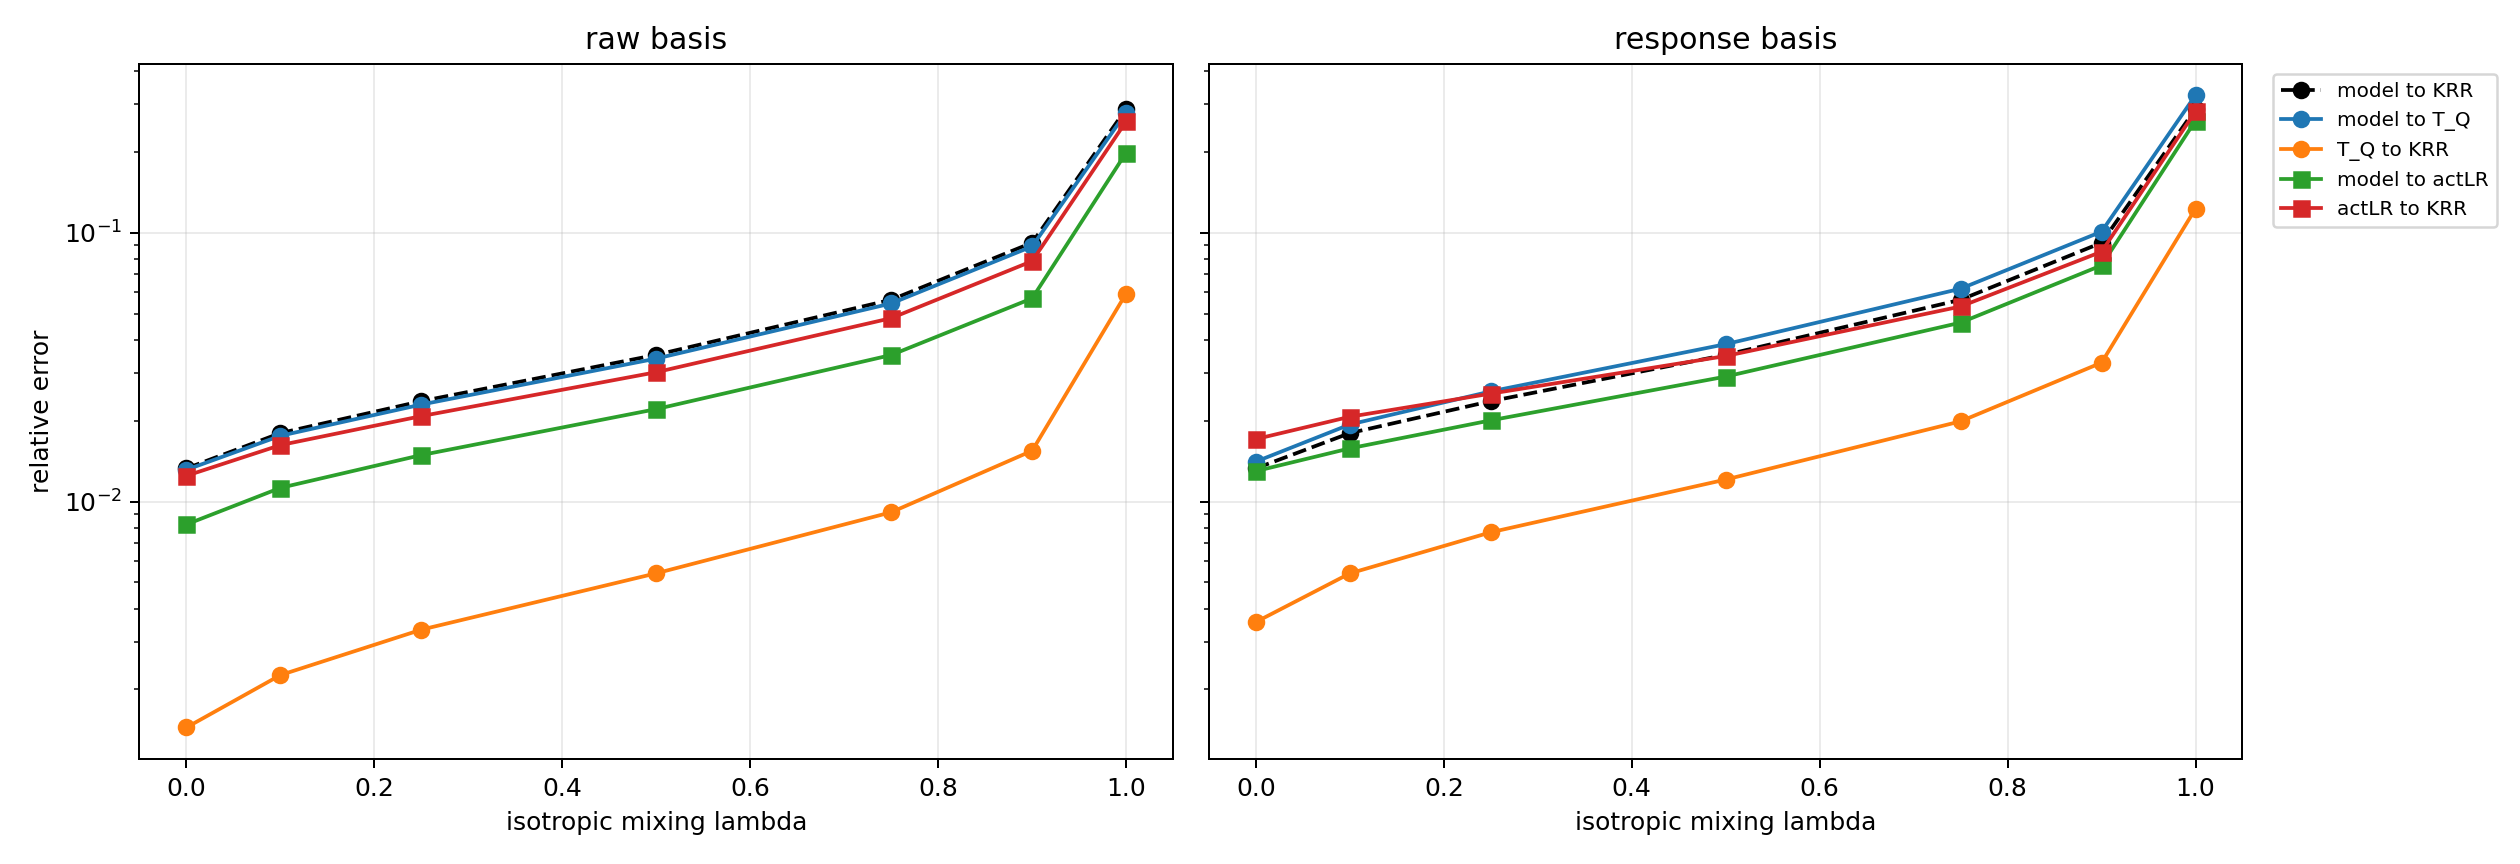
\includegraphics[width=\linewidth]{../experiments/exp1_operator_certificate/results/probe_interpolation.png}
\caption{Interpolation sweep from task-label probes to isotropic probes. The interpolation
parameter is \(\lambda\), with \(\lambda=0\) equal to task probes and \(\lambda=1\) equal to
isotropic probes. The reduced operator remains comparatively close to ridge while the
transformer's learned response drifts off distribution.}
\label{fig:interpolation}
\end{figure}

\begin{figure}[!htbp]
\centering
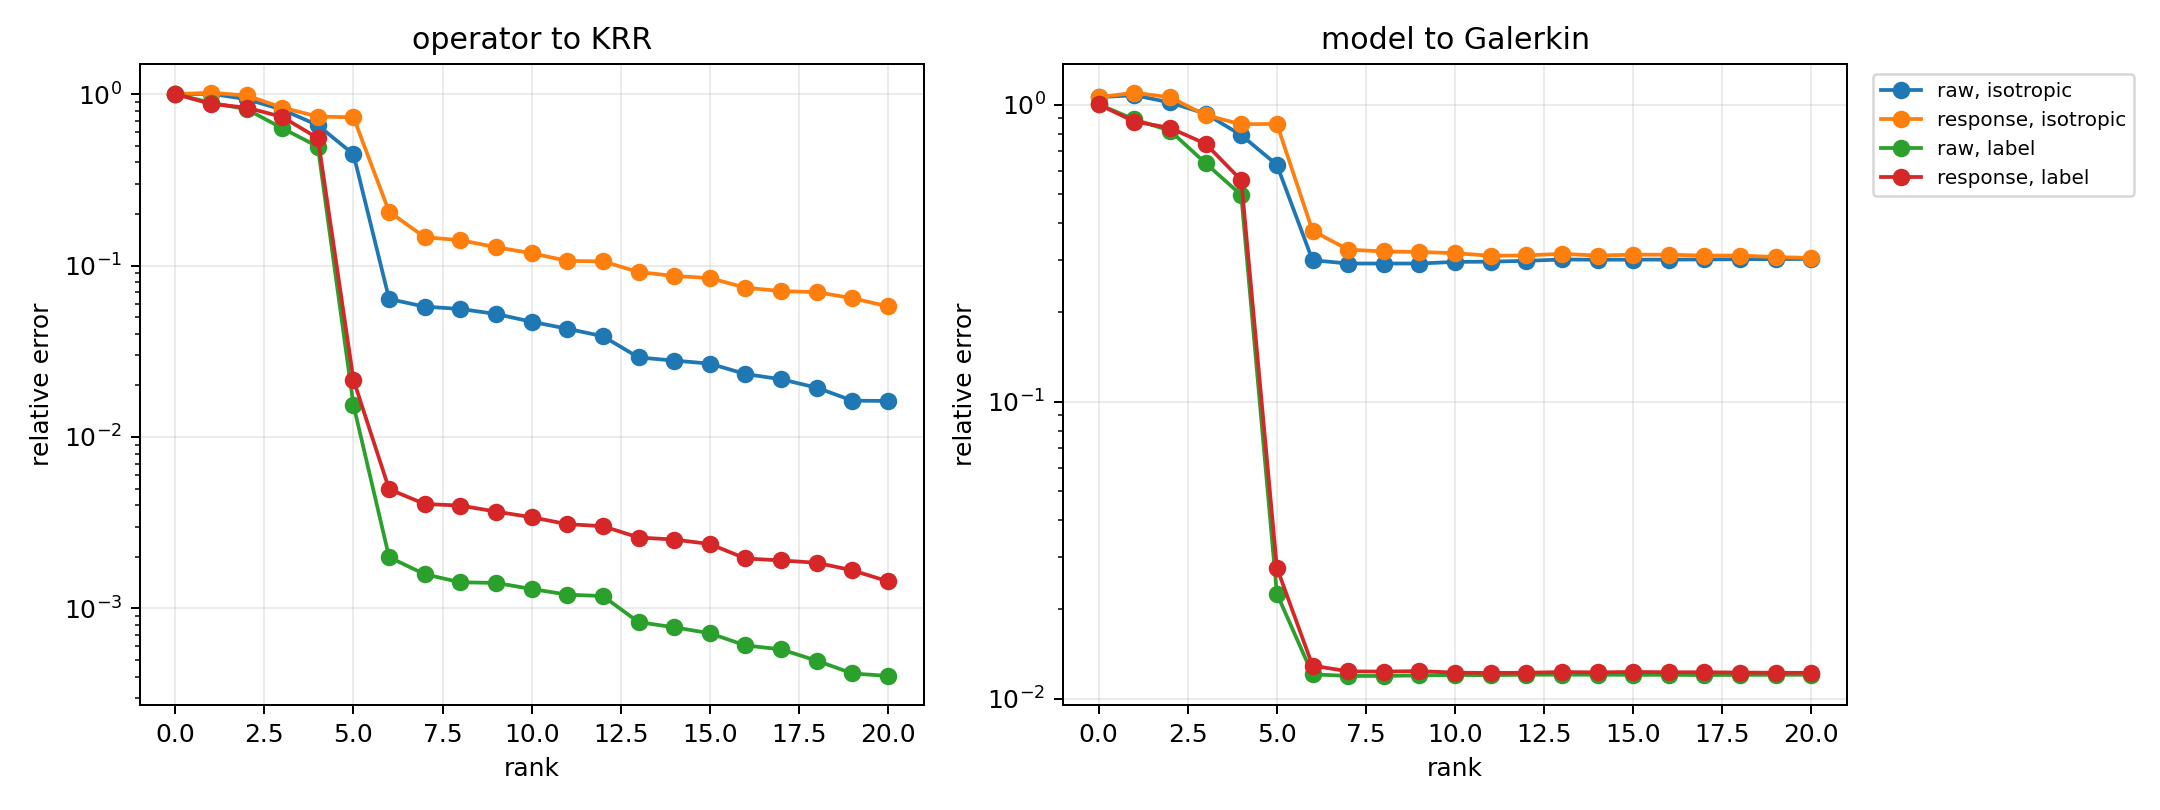
\includegraphics[width=\linewidth]{../experiments/exp1_operator_certificate/results/rank_curves.png}
\caption{Rank curves for the raw and response-only bases.}
\label{fig:rank-curves}
\end{figure}

\paragraph{Interpretation.}
Experiment 1 gives the endpoint certificate used by the rest of the note. On task-label
perturbations, the transformer is close to KRR, the raw final activation subspace induces a reduced
operator close to KRR, and the transformer is close to that reduced operator. The response-fitted
control shows that a better fitted readout from the same subspace is not automatically a better KRR
explanation: it improves transformer fit slightly but moves away from KRR. The random-subspace
controls show that the result is not a generic consequence of using a low-dimensional subspace of
the same rank. The isotropic probes show the limit of the claim: Experiment 1 certifies a task-local
operator explanation, not a global KRR implementation on all label directions. This experiment is
therefore the necessary endpoint check: without it, the layerwise and causal experiments could only
show that the transformer contains and uses some low-dimensional activation directions, not that
those directions realize the task-local KRR operator we want to explain.

\FloatBarrier

\subsection{Experiment 2: Causal Layerwise Rank and Task Rank}

\paragraph{Question.}
Does the layerwise activation span contain the task-visible directions needed for ridge regression?
Experiment 1 checked the endpoint: a final activation subspace can induce a reduced operator close
to exact KRR. Experiment 2 asks how this subspace is supplied across layers. In the linear task, the
required context-label dimension is the task-visible rank \(r_T\), which agrees with \(d_x\) in the
target-rank sweep. The question is therefore concrete: after we keep only directions that are both
visible in layerwise label responses and causally useful for the transformer response, does their
accumulated span reach \(r_T\)?

\paragraph{Procedure.}
For each episode, fix the sampled geometry and compute \(A=K+\sigma^2I\) and \(T=K_tA^{-1}\).
Draw four independent task-label probe sets: build probes, hidden-validation probes,
causal-selection probes, and held-out evaluation probes. The build probes propose candidate
directions, the causal-selection probes decide which candidates are accepted, and the
hidden-validation probes report closure diagnostics. The evaluation probes are used only after the
span is frozen.

At layer \(\ell\), compute hidden-response matrices \(M_\ell^{\mathrm{build}}\) and \(M_\ell^{\mathrm{val}}\)
from finite differences of the context-token hidden state. Suppose earlier layers have already
selected directions whose accumulated span before layer \(\ell\) has \(A\)-orthonormal basis
\(Q_\ell^{\mathrm{pre}}\). Remove the part already explained by this earlier span:
\[
N_\ell^{\mathrm{build}}
=
\left(I-Q_\ell^{\mathrm{pre}}(Q_\ell^{\mathrm{pre}})^\top A\right)M_\ell^{\mathrm{build}},
\qquad
N_\ell^{\mathrm{val}}
=
\left(I-Q_\ell^{\mathrm{pre}}(Q_\ell^{\mathrm{pre}})^\top A\right)M_\ell^{\mathrm{val}}.
\]
Thus \(N_\ell^{\mathrm{build}}\) is the novel label-sensitive layer response: it is what remains after
earlier accepted directions, propagated through the same \(A\)-geometry used by the reduced
operator, have been accounted for.

Candidate directions are obtained from the \(A\)-weighted SVD
\[
A^{1/2}N_\ell^{\mathrm{build}}=U_\ell\Sigma_\ell V_\ell^\top,
\qquad
q_i=A^{-1/2}U_{\ell,i}.
\]
The run keeps at most 16 candidates with singular value at least \(10^{-3}\sigma_1\). These
candidates are not automatically accepted. For each candidate \(q_i\), perform a causal removal
after layer \(\ell\): replace the context hidden state \(H_\ell^{\mathrm{ctx}}\) by
\[
H_\ell^{\mathrm{ctx}}
-
q_iq_i^\top AH_\ell^{\mathrm{ctx}},
\]
roll the remaining layers forward, and measure the finite-difference response damage on the
causal-selection probes:
\[
\Delta_\ell(q_i)
=
\frac{
\|D_\varepsilon F_{\ell,q_i}^{\mathrm{rem}}(y)-D_\varepsilon F(y)\|_F
}{
\|D_\varepsilon F(y)\|_F+\eta_{\mathrm{num}}
}.
\]
Here \(F_{\ell,q_i}^{\mathrm{rem}}\) denotes the transformer after removing direction \(q_i\) from the
context residual stream at layer \(\ell\). A candidate is accepted when \(\Delta_\ell(q_i)\ge 0.05\).
The accepted directions at all layers define \(Q_{\mathrm{lay}}\) through the layerwise activation-span
construction. Finally, freeze \(Q_{\mathrm{lay}}\), form
\(T_{Q_{\mathrm{lay}}}=K_tQ_{\mathrm{lay}}Q_{\mathrm{lay}}^\top\), and evaluate
\(E(T_{Q_{\mathrm{lay}}},T)\) and \(E_\varepsilon(F,T_{Q_{\mathrm{lay}}})\) on held-out task-label probes.

\paragraph{Results.}
The 16-episode target-rank sweep uses the causal selection rule described above. Let \(r_T\) be the
empirical task-visible rank of the ridge operator and let \(d_{\mathrm{lay}}=\dim R_{\mathrm{lay}}\). The
results are:

\begin{table}[ht]
\centering
\caption{Experiment 2 target-rank sweep with causal layerwise selection.}
\begin{tabular}{ccccccc}
\toprule
\(d_x\) & \(r_T\) & \(d_{\mathrm{lay}}\) & \(d_{\mathrm{lay}}/r_T\) &
\(E(T_{Q_{\mathrm{lay}}},T)\) & \(E(F,T)\) & \(E(F,T_{Q_{\mathrm{lay}}})\)\\
\midrule
3 & 3.0 & 3.0 & 1.000 & 0.0000 & 0.0063 & 0.0063\\
5 & 5.0 & 5.0 & 1.000 & 0.0000 & 0.0091 & 0.0091\\
8 & 8.0 & 8.0 & 1.000 & 0.0000 & 0.0129 & 0.0129\\
10 & 10.0 & 10.0 & 1.000 & 0.0000 & 0.0131 & 0.0131\\
15 & 14.9 & 14.5 & 0.971 & 0.0997 & 0.0174 & 0.1089\\
\bottomrule
\end{tabular}
\end{table}

For \(d_x=3,5,8,10\), the selected layerwise span reaches the task-visible rank and the reduced
operator is numerically exact on held-out task probes. For \(d_x=15\), the selected dimension
averages 14.5 while \(r_T\) averages 14.9, and the reduced-operator error rises to 0.0997. The
threshold is therefore visible in the held-out operator error: when the causal layerwise span reaches
\(r_T\), \(T_{Q_{\mathrm{lay}}}\) matches \(T\); when it remains slightly short, the reduced operator loses
accuracy. The held-out closure diagnostics follow the same pattern. The mean maximum validation
closure defect is about 0.027, 0.027, 0.026, 0.015 for \(d_x=3,5,8,10\), and rises to 0.110 for
\(d_x=15\).

The \(d_x=15\) case appears to fail for a simple reason: the selected span does not reliably recover
the last task-visible direction. This is the largest target-rank setting, so the required subspace is
nearly the full 15-dimensional feature span. The causal extraction often selects 14 rather than 15
independent directions, and the validation closure defect is higher, meaning that the accepted span
no longer covers all held-out layer responses. In the episodes where the selected span reaches the
full task-visible rank, the reduced-operator error is again numerical zero; the nonzero average error
comes from the episodes that miss one direction. Thus the failure is best read as incomplete rank
recovery by the layerwise extraction rule at the largest tested dimension, not as evidence that the
reduced-operator construction changes.

\begin{figure}[!htbp]
\centering
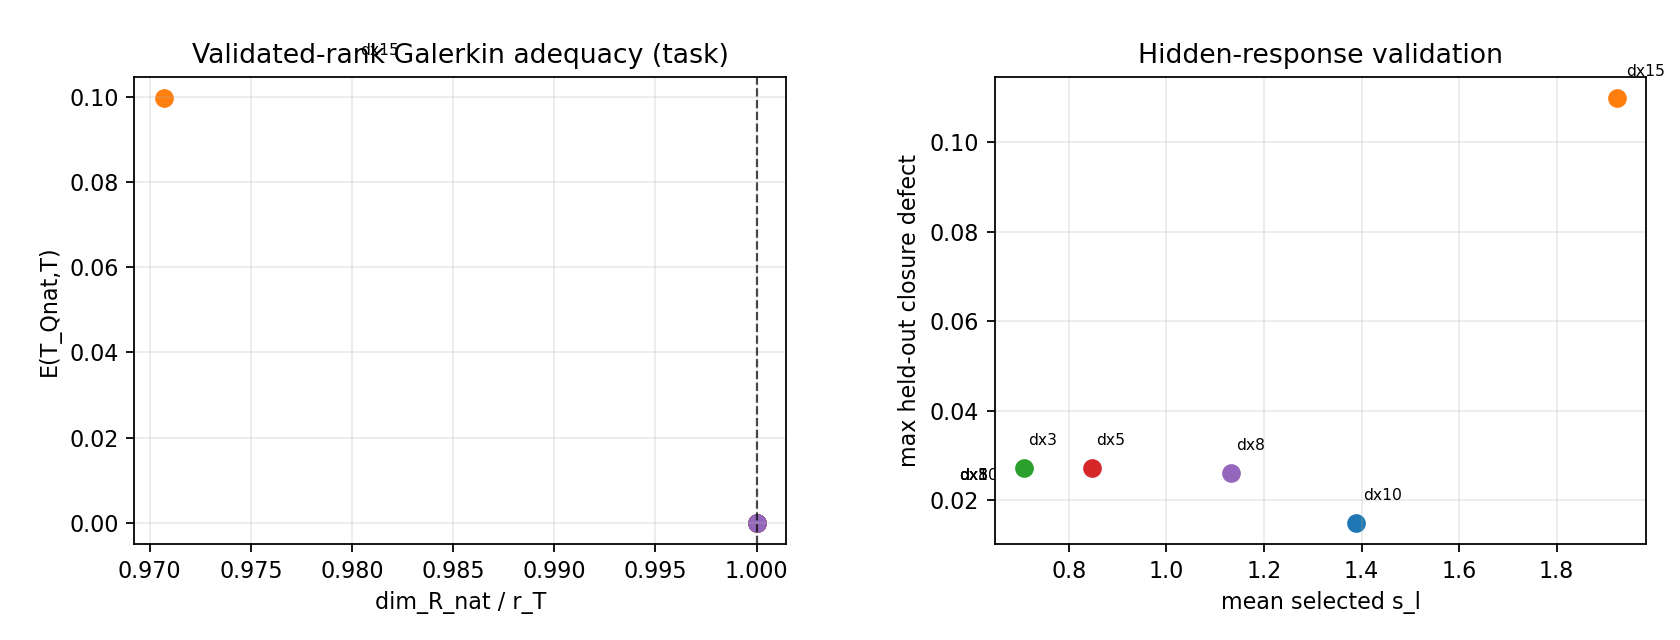
\includegraphics[width=0.92\linewidth]{../experiments/exp2_validated_rank/results_2b_causal_tau005_r16_nbuild16_ep16/causal_rank_task.png}
\caption{Experiment 2 target-rank sweep with causal layerwise selection. When the selected
layerwise dimension reaches the task-visible rank, the reduced-operator error collapses to
numerical zero. The \(d_x=15\) setting remains slightly under-ranked.}
\label{fig:target-rank-sweep}
\end{figure}

The depth/head sweep gives the necessary qualification. At fixed \(d_x=5\), causal selection gives
\(E(T_{Q_{\mathrm{lay}}},T)=0\) for all reported checkpoints, but transformer accuracy still varies. The
\(L=2\) checkpoint has \(d_{\mathrm{lay}}=20.6\) and exact reduced-operator error, yet \(E(F,T)=0.185\).
By contrast, the \(L=8\) checkpoint has \(d_{\mathrm{lay}}=5.0\), exact reduced-operator error, and
\(E(F,T)=0.0095\); the \(H=2\) and \(L=12\) checkpoints are similar, with transformer errors 0.0090
and 0.0094. The layerwise span therefore certifies availability of a subspace whose reduced
operator is ridge, not that the trained transformer's response is automatically accurate.

\paragraph{Interpretation.}
Experiment 2 supports a sharper resource law:
\[
d_{\mathrm{lay}}/r_T \approx 1
\quad\Longrightarrow\quad
E_{P_{\mathrm{task}}}(T_{Q_{\mathrm{lay}}},T)\approx 0.
\]
The law concerns the reduced operator induced by the causal layerwise span. It is not a statement
about raw architecture counts, and it is not by itself a statement about transformer accuracy.
This experiment was needed because Experiment 1 only showed that a suitable subspace is present
at the final state; it did not show whether the layerwise label responses supply the task-visible
number of directions. Experiment 2 shows that, for the linear task, the causally selected layerwise
span reaches exactly the dimension predicted by the KRR geometry in the successful target-rank
settings, and that operator error appears precisely when this span remains short.

\FloatBarrier

\subsection{Experiment 3: Causal Direction Removal}

\paragraph{Question.}
Are the task-important directions of the reduced operator causally used by the transformer? This is
needed because a direction can be decodable without being used. The surgery test removes
directions ranked important by the reduced operator and checks whether the transformer's
task-local response changes accordingly.

\paragraph{Procedure.}
For an extracted raw final \(A\)-orthonormal basis \(Q=[q_1,\ldots,q_r]\), define \(Q_{-j}\) by
removing column \(j\) from \(Q\). Direction \(q_j\) is important for the reduced operator if deleting
it changes the reduced operator's response. On a probe set \(U\), measure this by
\[
\Lambda_j^{\mathrm{red}}(U)
:=
\left(
\frac{
\sum_{u\in U}\|(T_Q-T_{Q_{-j}})u\|_2^2
}{
\sum_{u\in U}\|Tu\|_2^2+\eta_{\mathrm{num}}
}
\right)^{1/2}.
\]
Task leverage means this score computed on task-label probes; isotropic leverage means the same
score computed on isotropic probes. The main intervention set consists of the top-\(k\) directions
by task leverage.

We intervene on the context-token residual state after residual state \(s=0,\ldots,L\) by replacing
\[
H_s^{\mathrm{ctx}}
\longmapsto
H_s^{\mathrm{ctx}}
-
\sum_{j\in J}q_jq_j^\top AH_s^{\mathrm{ctx}},
\]
then roll the remaining layers forward. The intervention removes the \(A\)-orthogonal projection
of the context residual stream onto directions that the reduced operator predicts to be important.
Matched controls remove low-task-leverage directions from the same extracted basis,
high-isotropic-but-low-task directions, high-activation-variance-but-low-task directions, and random
subsets of \(Q\). The low-task directions are the cleanest negative control because they share the
same extraction pipeline and residual-stream coordinates.

\paragraph{Results.}
Before surgery the checkpoint is in the task-local reduced-operator regime:
\[
E_{\mathrm{task}}(F,T)=0.00926,\qquad
E_{\mathrm{task}}(F,T_Q)=0.00920,\qquad
E_{\mathrm{task}}(T_Q,T)=0.00086.
\]
The same episodes retain the off-distribution response drift seen above:
\[
E_{\mathrm{iso}}(F,T)=0.266,
\qquad
E_{\mathrm{iso}}(T_Q,T)=0.0378.
\]
Surgery is therefore applied in a regime where the task-local certificate holds before intervention.
At residual state \(s=1\), removing a single direction predicted to matter most for the reduced
operator causes prediction drift 4.68, KRR-error inflation \(649\times\), and task response damage
41.59. Removing a single low-task-leverage direction from the same basis is nearly inert:
prediction drift \(9.8\cdot 10^{-4}\), KRR-error inflation \(1.03\times\), and task response damage
0.0024.

The layer sweep localizes the effect. High-task surgery is most damaging at early residual states,
before later attention has routed the relevant context information into target tokens. Context-only
surgery after the final layer is a no-op, as expected from the architecture. At \(s=1\), the relationship
between aggregate task leverage and task response damage is strong across matched non-random
controls (log--log Pearson 0.91, Spearman 0.87). This is the key causal specificity check: damage
tracks task leverage, not merely activation energy or membership in the extracted subspace.

As a complementary mediation check, we also intervene on the whole extracted subspace at
residual state \(s=1\). Keeping only the \(A\)-projection of the context residual stream onto \(Q\),
\[
H_s^{\mathrm{ctx}}\mapsto QQ^\top AH_s^{\mathrm{ctx}},
\]
nearly preserves the task-local response: over 8 episodes,
\[
E_{\mathrm{task}}(F,T)=0.01866,
\qquad
\text{response damage}=0.01659.
\]
Removing the same subspace,
\[
H_s^{\mathrm{ctx}}\mapsto H_s^{\mathrm{ctx}}-QQ^\top AH_s^{\mathrm{ctx}},
\]
destroys the response:
\[
E_{\mathrm{task}}(F,T)=145.43,
\qquad
\text{response damage}=145.43.
\]
Thus, in this intervention family, the complement of \(Q\) is largely dispensable for the
task-local KRR response, while \(Q\) itself is necessary.

\begin{figure}[!htbp]
\centering
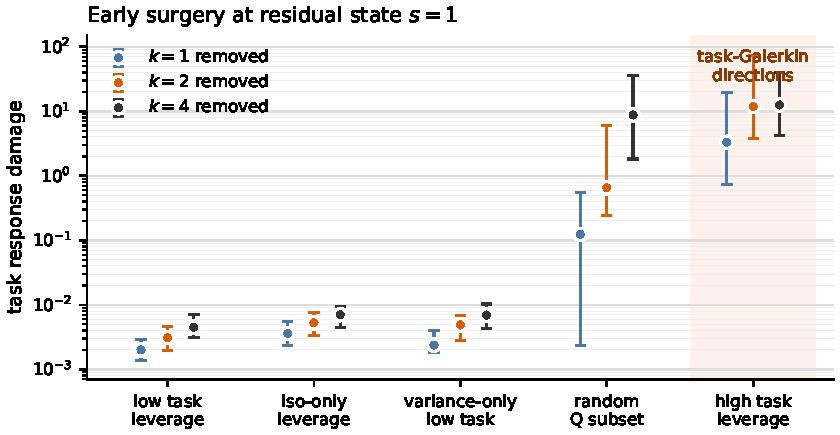
\includegraphics[width=0.78\linewidth]{../experiments/exp3_causal_surgery/results/experiment_3_key_surgery.pdf}
\caption{Experiment 3: causal effect of task-important activation directions. Task finite-difference
response damage after removing \(k\) context-token directions at residual state \(s=1\).
High task-leverage directions produce orders-of-magnitude larger damage than low-task-leverage
directions from the same activation basis.}
\label{fig:causal-direction-removal}
\end{figure}

\paragraph{Interpretation.}
The directions that the reduced operator identifies as task-relevant are not only decodable and
sufficient for small reduced-operator error; removing them before later attention can use them
strongly damages both prediction and the task-local finite-difference response.

\FloatBarrier

\section{Falsification and Conclusion}

The expected observation would be only that a transformer trained on linear regression gives
KRR-like predictions. That is not the main claim here. Pointwise prediction accuracy alone does
not identify the computation inside an in-context learner: many rules can agree on the sampled
labels while having a different response to nearby label perturbations.

The stronger claim is operator-level and task-local. After fixing the input geometry, KRR is the
linear map \(T=K_tA^{-1}\) from context labels to target predictions. We therefore ask whether the
transformer has the same local label-to-prediction response, whether that response can be explained
through a compact activation subspace, and whether the relevant directions in that subspace are
causally used.

The evidence has three parts. First, on held-out task-label perturbations, the transformer's
finite-difference response is close to the exact KRR operator. Second, the activation-derived subspace
becomes sufficient exactly when its dimension reaches the task-visible rank predicted from the KRR
spectrum. This rank is computed before looking at activations; it is the number of directions KRR
needs under the task label distribution. Third, the high-leverage directions of the reduced operator
are not merely decodable: removing them from the residual stream strongly damages prediction
and the task-local response, while matched low-leverage removals are nearly inert.

These observations make the result more specific than a generic low-rank explanation. The
same-span response-fitted low-rank control can fit the transformer's response slightly better on task
probes, but it agrees much worse with KRR. The reduced operator used here is constrained by the
KRR system itself, so success means that the extracted subspace supports the ridge computation,
not just that some low-rank response fit works after the fact.

The claim is also not global. Isotropic label probes show clear response drift: the transformer has
not learned a uniformly correct inverse on all possible label directions. The supported conclusion is
narrower and more mechanistic. On the label directions emphasized by the training distribution,
the trained transformer exposes a compact context-side activation subspace whose induced KRR
operator is accurate, whose required dimension is predicted by the task-visible rank, and whose
high-leverage directions are causally important for the transformer's response.

The account is falsifiable at each step. If \(E_\varepsilon(F,T)\) is large while pointwise error is small,
the transformer has not learned the conditional KRR response. If \(E(T_Q,T)\) is large, the extracted
subspace does not explain the KRR operator. If \(E(T_Q,T)\) is small but \(E_\varepsilon(F,T_Q)\) is
large, the subspace is sufficient but the transformer does not use it to produce its local response. If
\(T_{\mathrm{actLR}}\) explains held-out responses much better than \(T_Q\) while also staying close to
KRR, the reduced-operator construction is not the right explanation. If leverage does not predict
causal damage, the directions may be decodable but not causally operative.

\end{document}
